
% This LaTeX was auto-generated from MATLAB code.
% To make changes, update the MATLAB code and republish this document.

\documentclass{article}
\usepackage{graphicx}
\usepackage{color}

\sloppy
\definecolor{lightgray}{gray}{0.5}
\setlength{\parindent}{0pt}

\begin{document}

    
    
\section*{Ren� Nilsson - 10783 - Compulsory Assignment}


\subsection*{Contents}

\begin{itemize}
\setlength{\itemsep}{-1ex}
   \item Exercise 1
   \item Exercise 2
   \item Exercise 3
\end{itemize}


\subsection*{Exercise 1}

\begin{par}
Optimization using the simplex method:
\end{par} \vspace{1em}
\begin{verbatim}
% The augmented matrix:
clc; clear;
A = [1  2  0  1  0  0  0  28;
     2  0  4  0  1  0  0  16;
     0  1  1  0  0  1  0  12;
    -2 -5 -3  0  0  0  1  0]
\end{verbatim}

        \color{lightgray} \begin{verbatim}
A =

     1     2     0     1     0     0     0    28
     2     0     4     0     1     0     0    16
     0     1     1     0     0     1     0    12
    -2    -5    -3     0     0     0     1     0

\end{verbatim} \color{black}
    \begin{par}
We want to bring $x_2$ in, since $A(4,2) < A(4,3) < A(4,1)$, and thus increases $A(4,8)$ the most. The pivot row should be $A(3,2)$, since $$\frac{A(3,8)}{A(3,2)} = 12 < \frac{A(1,8)}{A(1,2)} = 14$\$
\end{par} \vspace{1em}
\begin{verbatim}
A(1,:) = A(1,:)-2*A(3,:);
\end{verbatim}
\begin{verbatim}
A(4,:) = A(4,:) + 5*A(3,:)
\end{verbatim}

        \color{lightgray} \begin{verbatim}
A =

     1     0    -2     1     0    -2     0     4
     2     0     4     0     1     0     0    16
     0     1     1     0     0     1     0    12
    -2     0     2     0     0     5     1    60

\end{verbatim} \color{black}
    \begin{par}
Next, we bring in $x_1$, since $A(4,1)$ is the only negative value in $A(4,:)$. $A(1,1)$ is the new pivot, since $$\frac{A(1,8)}{A(1,1)} = 4 < \frac{A(2,8)}{A(2,1)} = 8$\$
\end{par} \vspace{1em}
\begin{verbatim}
A(2,:) = A(2,:) -2*A(1,:);
\end{verbatim}
\begin{verbatim}
A(4,:) = A(4,:) + 2*A(1,:)
\end{verbatim}

        \color{lightgray} \begin{verbatim}
A =

     1     0    -2     1     0    -2     0     4
     0     0     8    -2     1     4     0     8
     0     1     1     0     0     1     0    12
     0     0    -2     2     0     1     1    68

\end{verbatim} \color{black}
    \begin{par}
Last, we bring in $x_3$, with pivot $A(2,3)$, since $A(1,3)$ is negative and $$\frac{A(2,8)}{A(2,1)} = 1 < \frac{A(3,8)}{A(3,1)} = 12$\$
\end{par} \vspace{1em}
\begin{verbatim}
A(2,:) = A(2,:)/8;
\end{verbatim}
\begin{verbatim}
A(1,:) = A(1,:) + 2*A(2,:);
\end{verbatim}
\begin{verbatim}
A(3,:) = A(3,:) - A(2,:);
\end{verbatim}
\begin{verbatim}
A(4,:) = A(4,:) + 2*A(2,:)
\end{verbatim}

        \color{lightgray} \begin{verbatim}
A =

  Columns 1 through 7

    1.0000         0         0    0.5000    0.2500   -1.0000         0
         0         0    1.0000   -0.2500    0.1250    0.5000         0
         0    1.0000         0    0.2500   -0.1250    0.5000         0
         0         0         0    1.5000    0.2500    2.0000    1.0000

  Column 8

    6.0000
    1.0000
   11.0000
   70.0000

\end{verbatim} \color{black}
    \begin{par}
Thus the maximum of the problem is 70, which is achieved when $x_1 = 6$, $x_2 = 1$ and $x_3 = 11$.
\end{par} \vspace{1em}


\subsection*{Exercise 2}

\begin{par}
Minimizing the function $f(x) = x_1^2+3*x_2^2-2*x_1*x_2+3*x_2$. 1. Write f on the form: $\frac{1}{2}*x^T*Q*x-x^T*b$:
\end{par} \vspace{1em}
\begin{verbatim}
Q = [2 -2;-2 6]
b = [0;-3]
\end{verbatim}

        \color{lightgray} \begin{verbatim}
Q =

     2    -2
    -2     6


b =

     0
    -3

\end{verbatim} \color{black}
    \begin{par}
2. Sketch the levels set for f and the gradient of f in the point $(1,1)^T$ in a $x_1,x_2$-coordinate system.
\end{par} \vspace{1em}
\begin{verbatim}
[x1, x2] = meshgrid(-10:1:10,-10:1:10);
x = [x1;x2];
f1 = x1.^2+3*x2.^2-2*x1.*x2+3*x2;
[C,h1] = contour(x1,x2,f1,[0 3 10 50 100 200 400]);
set(h1,'ShowText','on','TextStep',get(h1,'LevelStep')*2)
colormap cool
title('Level sets of f (x)')
xlabel('x1')
ylabel('x2')
\end{verbatim}

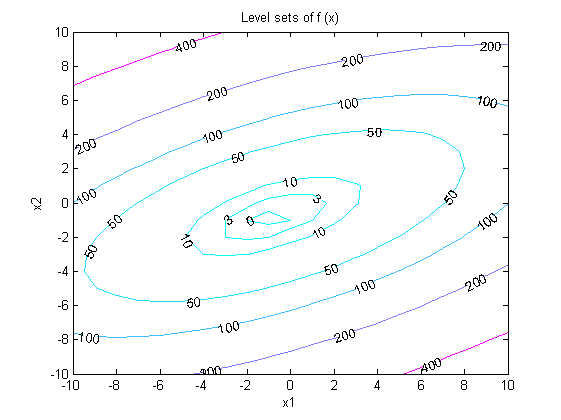
\includegraphics [width=4in]{Assignment10783_01.png}
\begin{par}
Gradient of f in the point $(1,1)^T$:
\end{par} \vspace{1em}
\begin{verbatim}
g1 = Q*[1;1]-b
\end{verbatim}

        \color{lightgray} \begin{verbatim}
g1 =

     0
     7

\end{verbatim} \color{black}
    \begin{par}
3. Find all point satisfying the FONC. Do these points satisfy the SONC?
\end{par} \vspace{1em}
\begin{par}
The gradient of f is found to be: $$f'(x)= Q*x-b$\$
\end{par} \vspace{1em}
\begin{par}
Finding the point satisfying the FONC equals solving the following: $$Q*x-b = 0$\$
\end{par} \vspace{1em}
\begin{par}
This gives the following point:
\end{par} \vspace{1em}
\begin{verbatim}
x = inv(Q)*b
\end{verbatim}

        \color{lightgray} \begin{verbatim}
x =

   -0.7500
   -0.7500

\end{verbatim} \color{black}
    \begin{par}
The Hessian is found to be $F(x) = Q$. Thus, the SONC is to test whether Q \ensuremath{>} 0:
\end{par} \vspace{1em}
\begin{verbatim}
format short
eigs(Q)
\end{verbatim}

        \color{lightgray} \begin{verbatim}
ans =

    6.8284
    1.1716

\end{verbatim} \color{black}
    \begin{par}
Since all eigenvalues of Q is positive, Q \ensuremath{>} 0 then the SONC is satisfied in all points satisfiying the FONC.
\end{par} \vspace{1em}
\begin{par}
4. Find the minimum of f over $R^2$
\end{par} \vspace{1em}
\begin{par}
Since both the FONC and SOSC is satisfied by the previous piont, this is the global minimum:
\end{par} \vspace{1em}
\begin{verbatim}
x
\end{verbatim}

        \color{lightgray} \begin{verbatim}
x =

   -0.7500
   -0.7500

\end{verbatim} \color{black}
    

\subsection*{Exercise 3}




\end{document}
    
